\documentclass[12pt]{article}
\usepackage{newlfont}
\usepackage{graphicx}
\usepackage{amssymb}

\title{Introduction to Algorithms, 2ed 's Notes}
\author{Bui Hong Ha}
\date{\today}

\begin{document}
\maketitle
\begin{abstract}
This is notes of my self-study course on Algorithms. It's taken when I was read the book "Introduction to Algorithms, 2ed"
\addcontentsline{toc}{section}{abstract}
\end{abstract}

\tableofcontents

\section{String Matching}
\subsection{String matching with finite automata}
\textbf{Finite automata}\\
A finite automaton M is a 5-tuple $ (Q,q_0, A, \Sigma, \delta) $, where
\begin {itemize}
	\item Q is a finie set of \textbf{\textit{states}}
	\item $ q_0 \in Q $ is the \textbf{\textit{start state}}
	\item $ A \subseteq Q $ is a distinguished set of \textbf{\textit{accepting states}}
	\item $ \Sigma $ is a finite \textbf{\textit{input alphabet}}
	\item $ \delta $ is a function from $ Q \times \sum \rightarrow Q $, called the \textbf{\textit{transition function}} of M.
\end {itemize}  

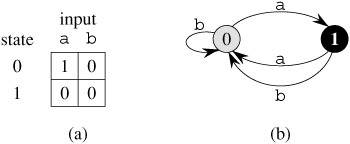
\includegraphics[width=100mm]{simple_2_states_automaton.jpg} 
\\

\textbf{Final-state function}\\
A finite automaton $M$ induces a function $\phi$, called the \textbf{\textit{final-state function}}, from $\Sigma^*$ to $Q$ such that $\phi (w)$ is the state $M$ ends up in after scanning the string $w$. Thus, $M$ accepts a string w if and only if $\phi (w) \in A $. The function $\phi $ is defined by the recursive relation
\begin{eqnarray*}
	\phi (\epsilon) & = & q_0
 	\\ \phi (wa) & = & \delta (\phi (w),a) \mbox{ for } w \in \Sigma^{*}, a \in \Sigma 
\end{eqnarray*} 
\\
\textbf{Suffix Function}\\
We define an auxiliary function $ \sigma $, called the \textbf{\textit{suffix function}} corresponding to P. The function $ \sigma $ is a mapping from $ \sum^{\ast} \rightarrow \{0,1,\ldots,m\} $ such that $ \sigma (x) $ is the length of the longest prefix of P that is suffix of x:\\
$ \sigma (x) = max \{k:P_k \sqsupset x\} $ \\
For example: for the pattern $ P = ab $ we have $ \sigma (\epsilon) = 0, \sigma (ccaca) = 1, \mbox{ and, } \sigma(ccab)=2 $ \\ \\
We define the string-matching automaton that corresponds to a given pattern $P[1\ldots m] $ as follows.
\begin{itemize}
	\item The state set $ Q $ is $ \{0,1,\ldots,m\}$. The start state $q_0$ is state 0, and state $m$ is the only accepting state
	\item The transition function $\delta$ is defined by the following equation, for any state $q$ and character a: \\
	$ \delta (q,a) = \sigma (P_{q}a) $
\end{itemize}

After scanning the first $i$ characters of the text string T, the machine is in state $\phi (T_i) = q$, where $q = \sigma(T_i)$ is the length of the longest suffix of $T_i$ that is also a prefix of the pattern $P$. If the next character scanned is $T[i+1] = a$, then the machine should make a transition to state $\sigma(T_{i+1}) = \sigma(T_i a)$. Theorem shows that $\sigma(T_i a) = \sigma(P_q a)$. That is, to compute the length of the longest suffix of $T_i a$ that is a prefix of $P$, we can compute the longest suffix of $P_q a$ that is a prefix of P. At each state, the machine only needs to know the length of the longest prefix of $P$ that is a suffix of what has been read so far. Therefore, setting $\delta(q,a) = \sigma(P_q a)$ maintains the desired invariant
\\ \\
\textbf{The Knuth-Morris-Pratt algorithm}

This algorithm avoids the computation of the transition function $\delta$ altogether, and its matching time is $\ominus (n)$ using just an auxiliary function $\pi[1 \ldots m]$ precomputed from the pattern in time $\ominus (m)$. 
\end{document}
